\section{Robustness Within the Tested Envelope}
\label{sec:robustness-results}

\subsection{Frozen condition-wise holdout}

The local-polynomial candidate was selected using development seeds only and then frozen. On the holdout, all \ESeventeenWorkPairCount{} paired cells improve normalized velocity ripple, and all 11 declared conditions pass their condition-wise criteria. The aggregate near-unity reductions under clean, quantized, delayed, dropout, and timestamp-jitter inputs are less informative than the weakest condition. At position noise $0.1$ of a position step, the median reduction is \ESeventeenWeakMedianPercent, the minimum across paired cells is \ESeventeenWeakMinimumPercent, and all \ESeventeenPairPerCondition{} pairs still improve. Reporting this weakest result avoids allowing easy conditions to dominate a pooled median.\claimtag{C6}

\begin{figure*}[t]
 \centering
 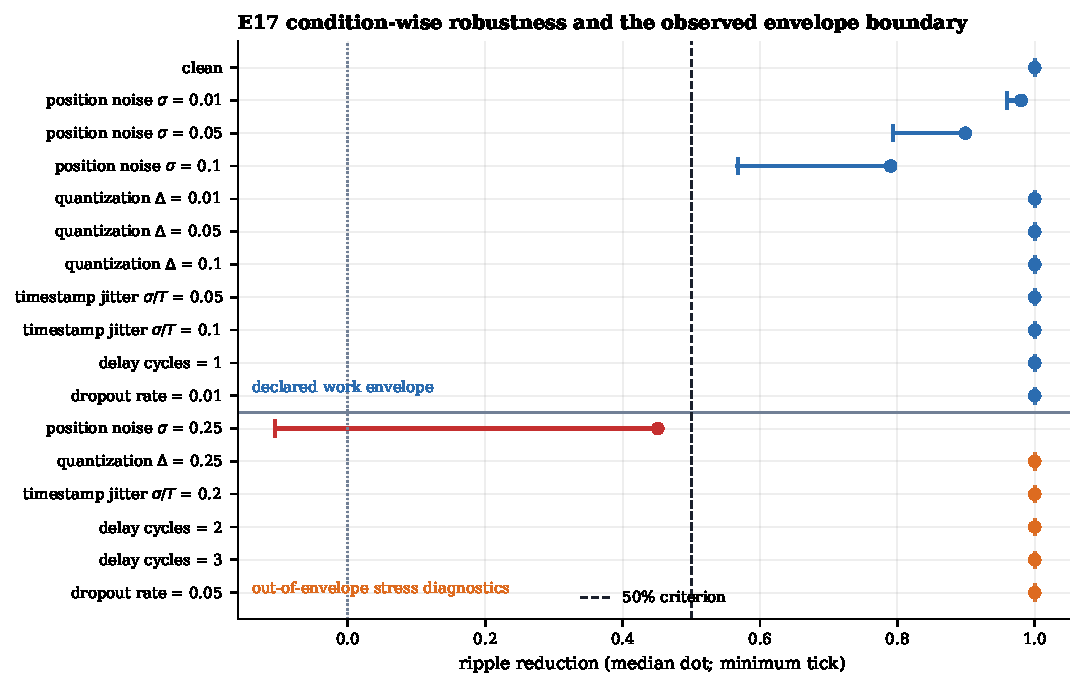
\includegraphics[width=\textwidth]{figures/generated/fig5_e17_robustness.pdf}
 \caption{E17 condition-wise results. Dots show medians and ticks show minima over \ESeventeenPairPerCondition{} paired seed--configuration cells per condition. The first 11 rows form the declared work envelope. The remaining six rows are stronger stress diagnostics. Position noise $0.25$ crosses the 50\% median criterion and contains one cell with negative reduction, exposing an observed boundary rather than supporting extrapolation.}
 \label{fig:e17-robustness}
\end{figure*}

The paired design matters. E17 contains \ESeventeenHoldoutRowCount{} holdout method rows because it evaluates multiple candidate methods and baselines, but those rows are not independent tasks. The confirmatory statement uses matched baseline--candidate pairs indexed by perturbation, $q$, $\rho$, and seed. We report exact condition counts and distributions rather than treating all internal rows as independent samples or highlighting a bootstrap interval across pseudo-replicated solver calls.

\subsection{Stress diagnostics expose the envelope boundary}

The six stronger perturbations were retained precisely to test how the selected observer fails outside the declared envelope. Five remain near complete ripple suppression. Position noise $0.25$, however, has median reduction \ESeventeenStressMedianPercent, below the $50\%$ condition criterion, and a minimum of \ESeventeenStressMinimumPercent. Although \ESeventeenStressImprovedCount{} of \ESeventeenPairPerCondition{} cells still improve, one becomes worse than its P-only baseline. This is not a failed preregistered holdout because the condition was never in the work envelope. It is a useful domain boundary that constrains the claim: the causal PV construction is robust \testedEnvelope, not under arbitrary position noise.\claimtag{C6}

The result also separates the target-state remedy from observer quality. Proposition~\ref{prop:matched-pv} assumes a matched velocity is available. A noisy causal estimator may fail to supply it closely enough. The resulting loss of performance does not reinstate the zero-velocity P-only contract as correct; it shows that derivative estimation and target semantics are two different design problems.

\subsection{Nonconstant synthetic trajectories}

All \ESeventeenSyntheticCount{} held-out synthetic trajectories pass the trajectory-level guardrails. They cover constant, ramp, sine, chirp, and reversal families, and the worst ripple reduction is \ESeventeenSyntheticWorstPercent. This extends the observed mechanism beyond constant schedules in the tested generator: carrying a causal velocity target remains beneficial when the intended derivative varies smoothly and changes sign.\claimtag{C7}

The extension remains synthetic. The trajectories share the single-axis kinematic model and generated disturbance process. They do not contain robot dynamics, contact, coupled joint limits, synchronization, sensor calibration errors, or a task distribution sampled from deployed robots. We therefore avoid terms such as robot generalization. The correct description is a nonconstant synthetic holdout inside a declared experimental design.

\subsection{Irregular timestamps: a visible negative result}

The recorded replay has source intervals from approximately $8.98$ to $11.09$ ms. Fixed-grid \FutureOOne{} rejects this horizon because it supports exactly one nominal step, which is the safe behavior under the information contract. The timestamp-aware local-polynomial method completes, but its RMSE is \RecordedLocalPolyRMSE, worse than the scheduled-P value \RecordedBaselineRMSE. It also leaves the same 20 ms integer observed lag. This replay is not an independent holdout and does not overturn the fixed-grid A04 result; it shows that the current irregular-timestamp observer has not solved the recorded case.\claimtag{C13}

\Cref{tab:robustness} consolidates the work-envelope result, the separately
labeled stress diagnostics, the synthetic trajectories, and this negative
replay without pooling their statistical units.
